\section{Demo hệ thống}
Nhóm xây dựng hệ thống Dashboard tương tác giúp người dùng theo dõi và phân tích thị trường Crypto. Hệ thống được triển khai trên nền tảng \textit{Streamlit} (Python + Plotly), kết nối trực tiếp với PostgreSQL Database (Gold Layer) hoặc đọc trực tiếp từ các tệp CSV xuất từ tầng Gold (chế độ ``CSV mode'' qua \texttt{streamlit\_crypto\_csv.py}).

\subsection{Giao diện Dashboard Streamlit}
Giao diện được thiết kế theo phong cách Dark Theme với 5 tab chức năng chính tương ứng với năm góc nhìn phân tích khác nhau.

\begin{figure}[H]
    \centering
    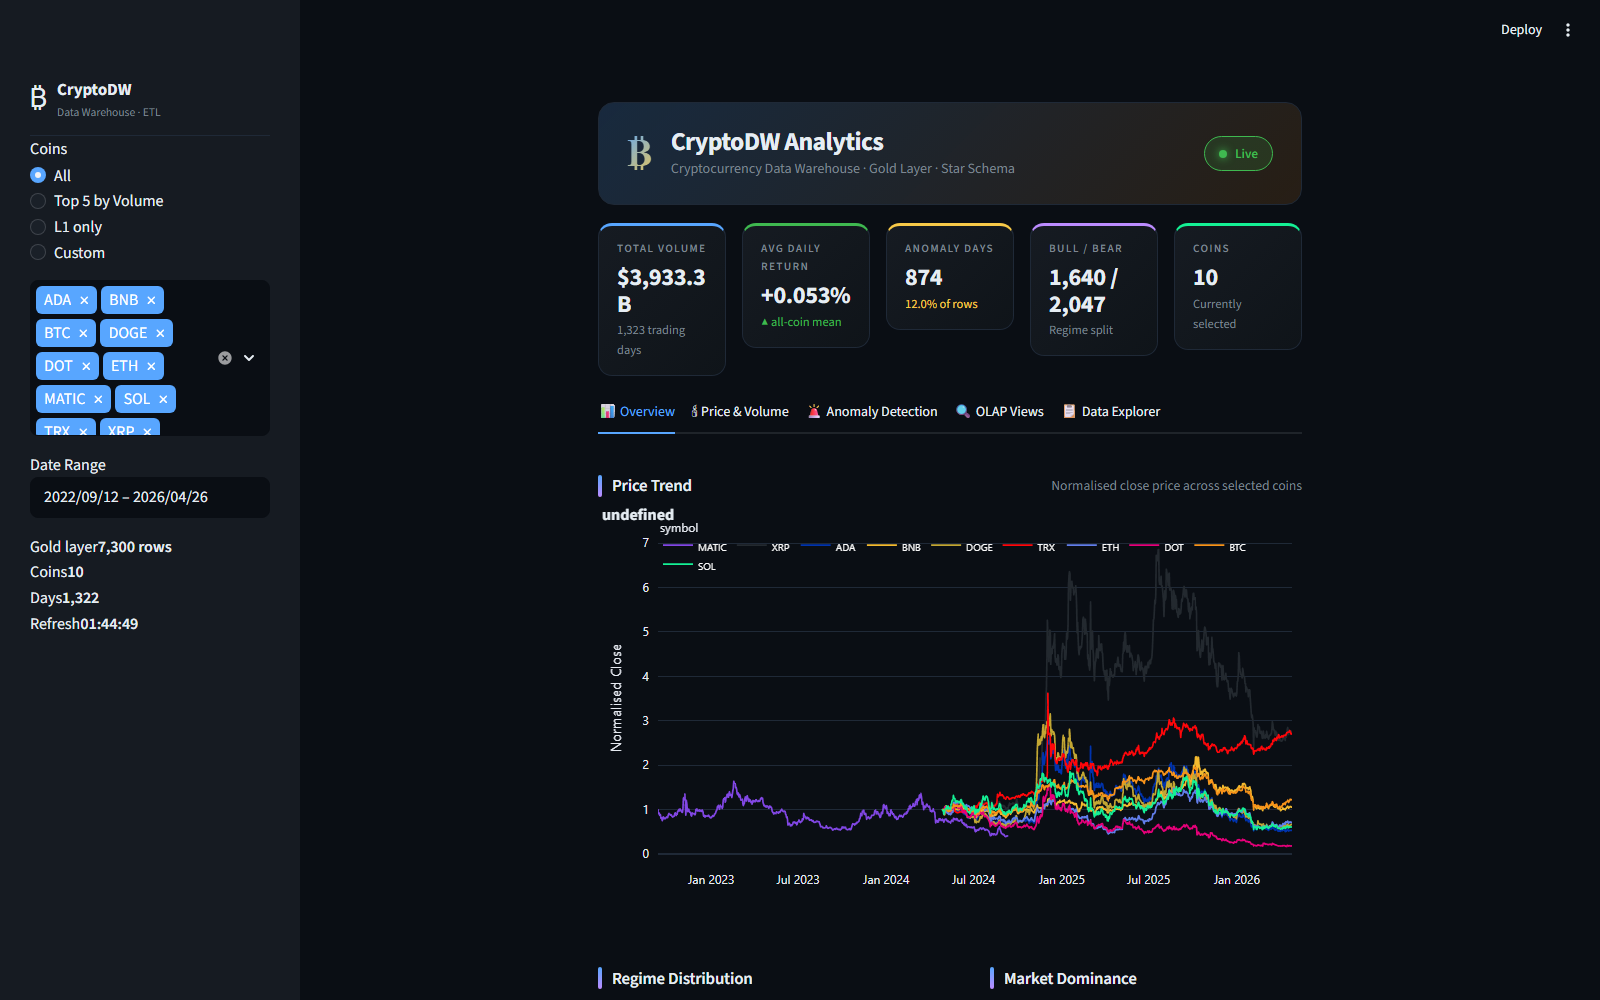
\includegraphics[width=1.0\textwidth]{Images/Demo/Main interface.png}
    \caption{Tab \textbf{Overview} -- Tổng quan thị trường: KPI bar (Total Volume, Avg Daily Return, Anomaly Days, Bull/Bear Days, Coins Selected) và Daily Close Price chart cho toàn bộ 10 đồng coin.}
    \label{fig:demo_overview}
\end{figure}

\begin{figure}[H]
    \centering
    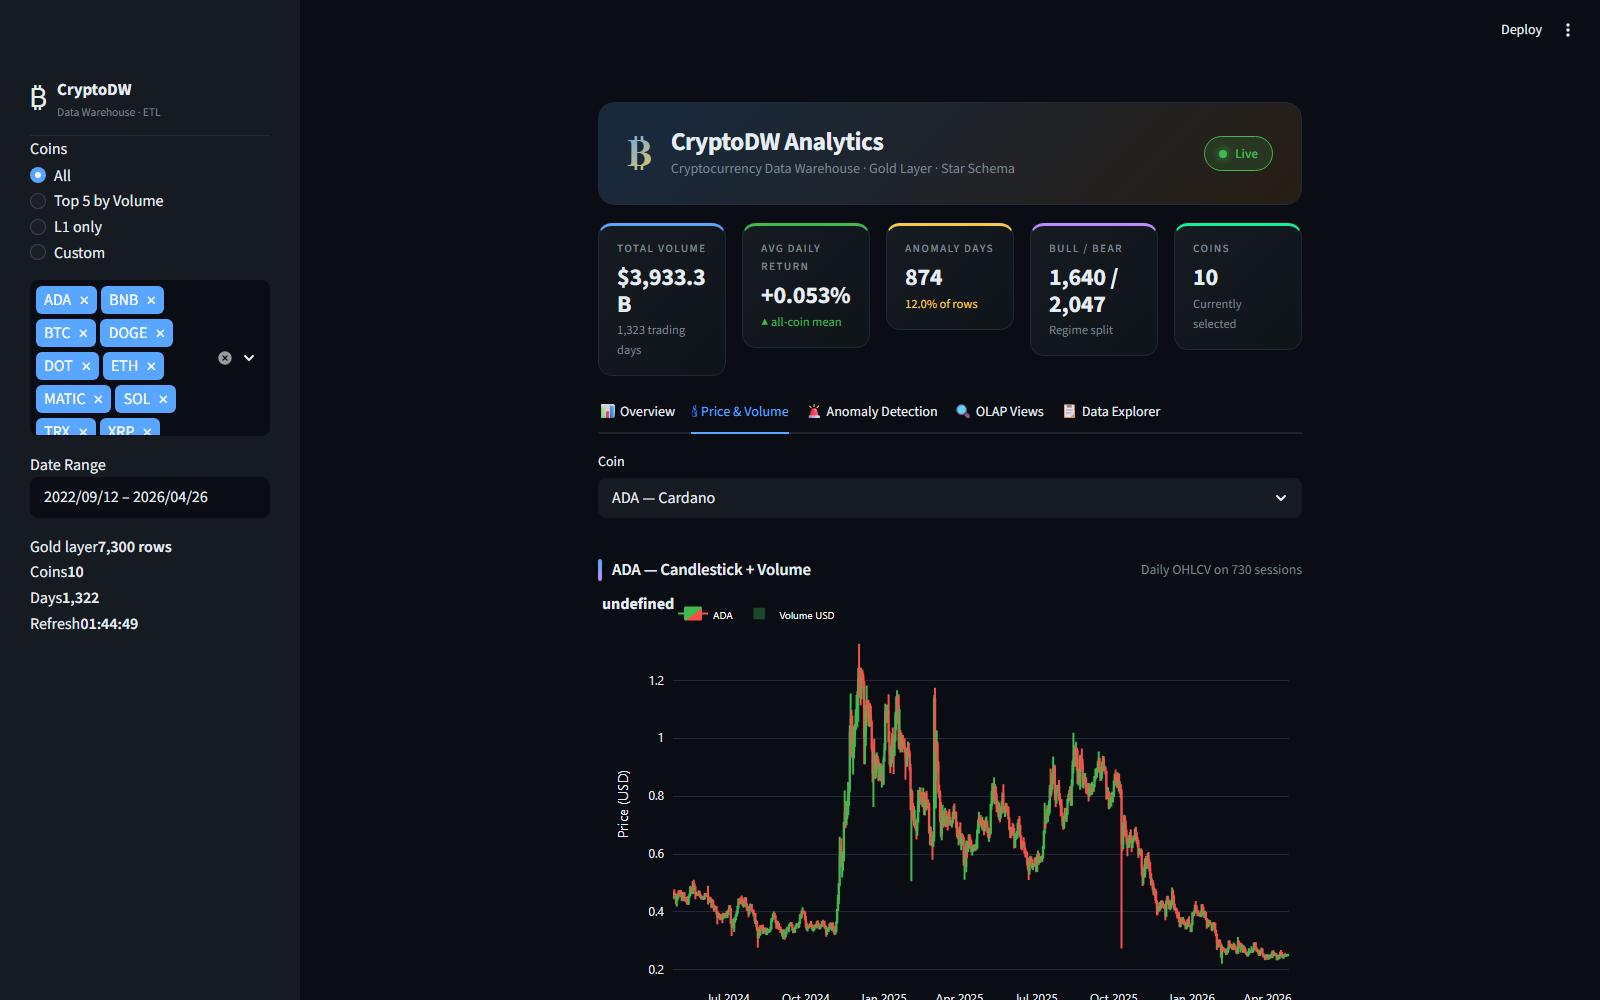
\includegraphics[width=1.0\textwidth]{Images/Demo/Visualize.png}
    \caption{Tab \textbf{Price \& Volume} -- Candlestick chart kèm volume bars cho từng coin, có Return Distribution histogram và Volatility timeline.}
    \label{fig:demo_price}
\end{figure}

\begin{figure}[H]
    \centering
    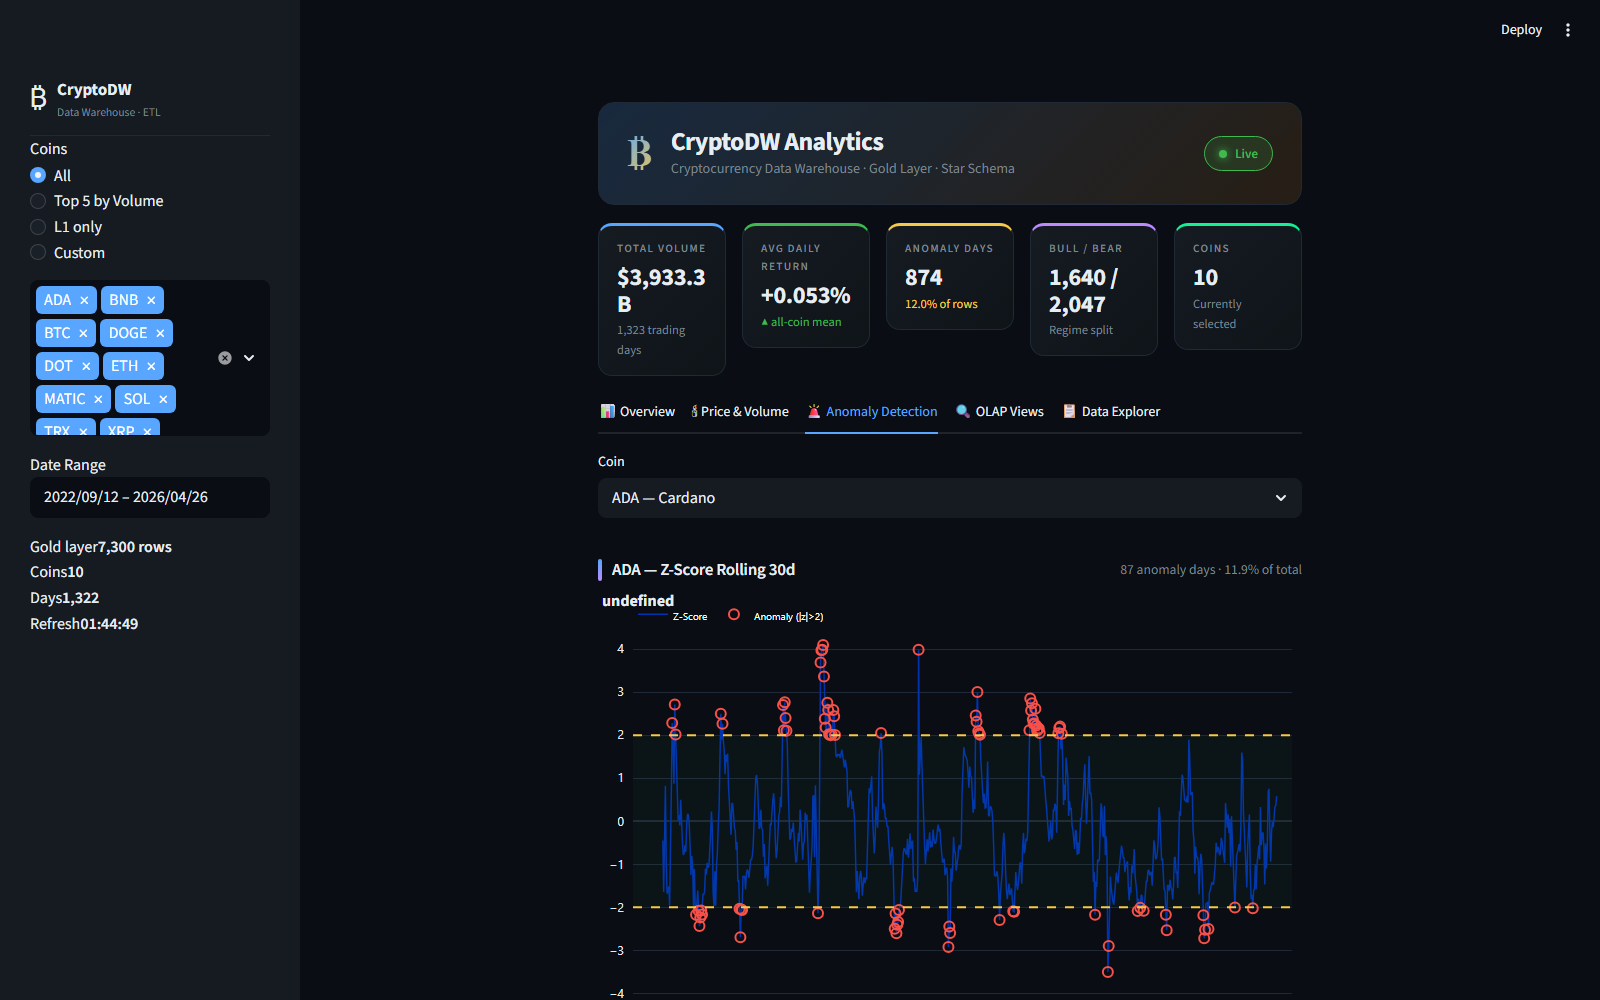
\includegraphics[width=1.0\textwidth]{Images/Demo/Detection.png}
    \caption{Tab \textbf{Anomaly Detection} -- Z-Score rolling 30 ngày với các phiên anomaly ($|z|>2$) đánh dấu đỏ, kèm Anomaly Rate per Coin và bảng Top 10 Extreme Anomalies.}
    \label{fig:demo_anomaly}
\end{figure}

\begin{figure}[H]
    \centering
    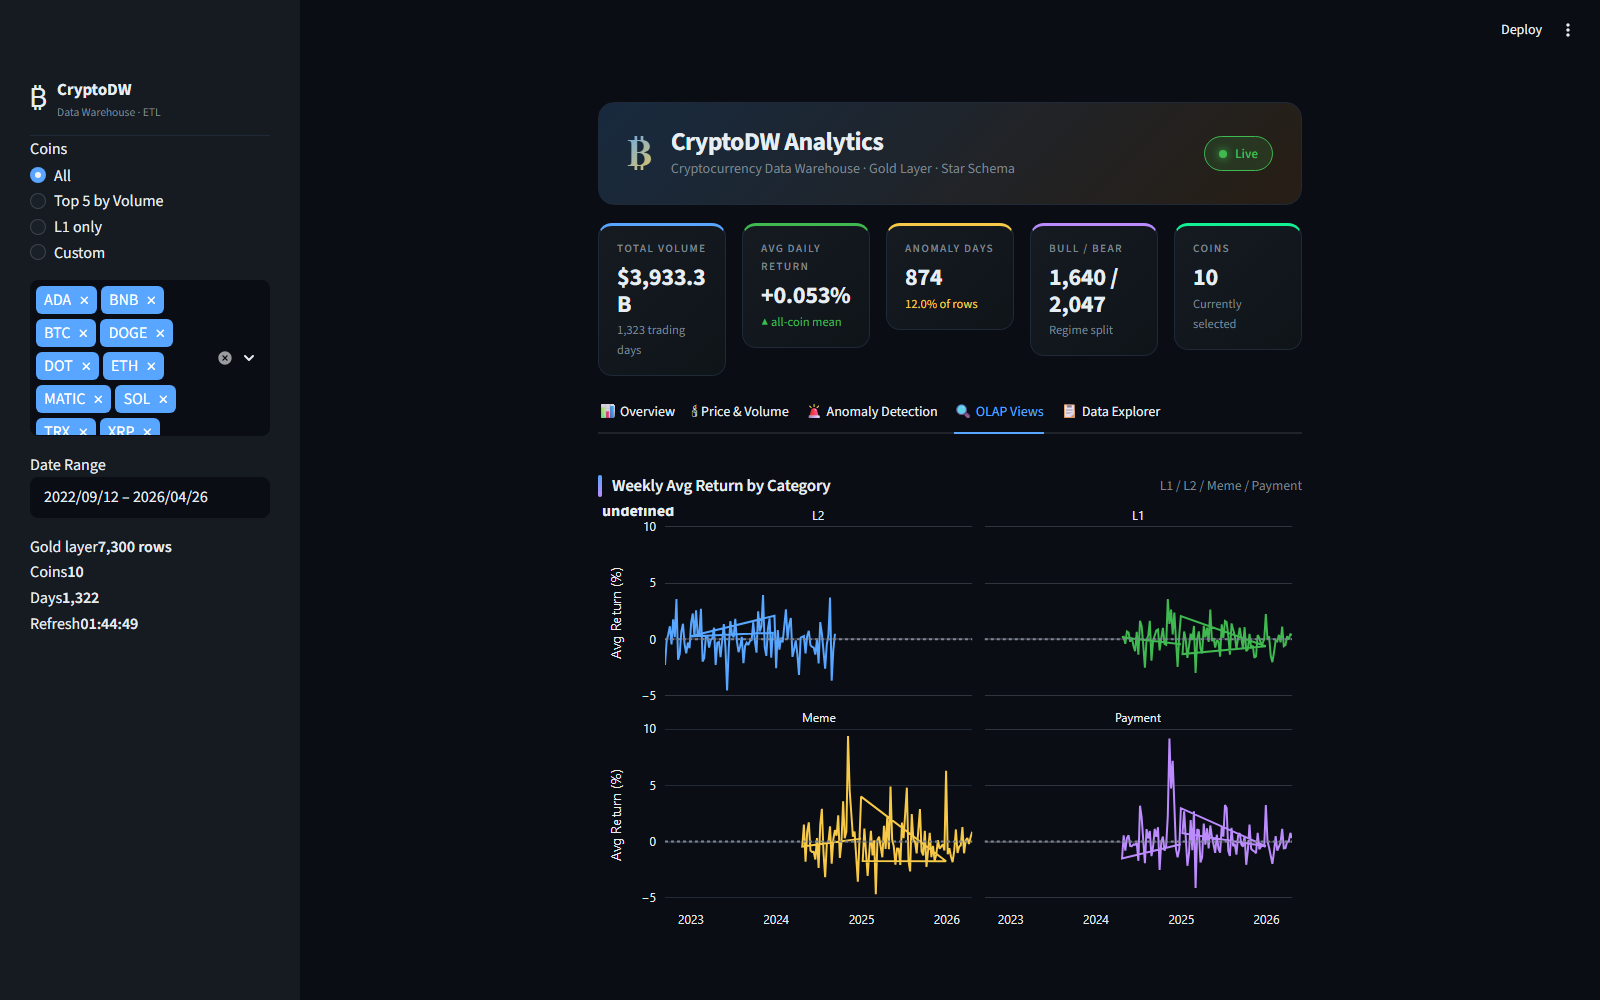
\includegraphics[width=1.0\textwidth]{Images/Demo/Individual ticker analysis.png}
    \caption{Tab \textbf{OLAP Views} -- Weekly Avg Return facet theo Category (L1/L2/Meme/Payment), Correlation Heatmap và Volume Leaderboard.}
    \label{fig:demo_olap}
\end{figure}

\begin{figure}[H]
    \centering
    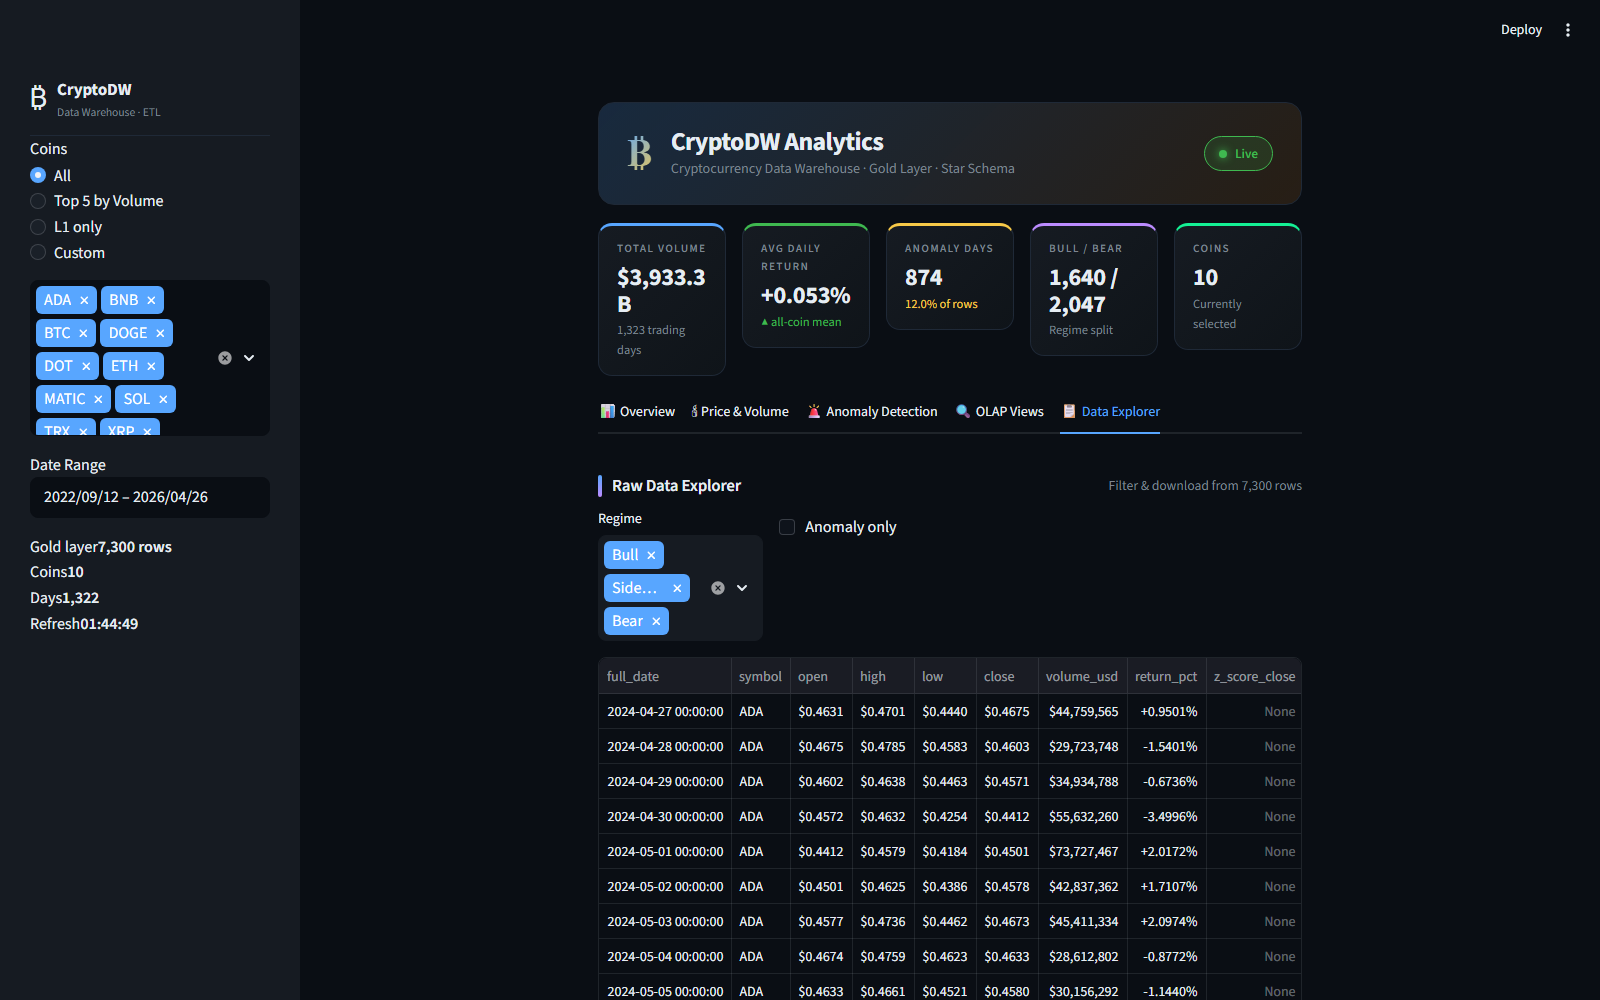
\includegraphics[width=1.0\textwidth]{Images/Demo/Upload.png}
    \caption{Tab \textbf{Data Explorer} -- Bảng dữ liệu thô với filter theo Regime/Anomaly, hỗ trợ download CSV.}
    \label{fig:demo_data}
\end{figure}

\subsection{Kịch bản Demo}
Quy trình demo hệ thống bao gồm 4 bước chính:
\begin{enumerate}
    \item \textbf{Cập nhật dữ liệu:} Chạy \texttt{run\_pipeline.bat} (Windows) hoặc \texttt{run\_pipeline.sh} (Linux/WSL) để kích hoạt luồng ETL: Binance API $\rightarrow$ Staging $\rightarrow$ Transform $\rightarrow$ Gold Layer $\rightarrow$ refresh OLAP views.
    \item \textbf{Phân tích OLAP:} Sử dụng tab Overview và Price \& Volume để slice/dice theo coin và khoảng thời gian; quan sát Market Dominance, Regime Distribution và Volume Leaderboard.
    \item \textbf{Khai phá dữ liệu:} Truy cập tab Anomaly Detection để xem các phiên có $|z\_score| > 2$. Mở Jupyter notebooks trong thư mục \texttt{ai/} để xem kết quả Linear Regression, K-Means clustering và Anomaly Detection ở mức code chi tiết.
    \item \textbf{Báo cáo quản trị:} Mở Power BI Dashboard (\texttt{bi/Crypto\_Dashboard.pbix}) để xem báo cáo tổng hợp theo quý và năm.
\end{enumerate}

\subsection{CSV mode -- chạy không cần PostgreSQL}
Để hỗ trợ giảng viên/đồng nghiệp chạy thử nhanh mà không cần cài đặt PostgreSQL, nhóm bổ sung script \texttt{streamlit\_crypto\_csv.py} đọc trực tiếp 4 tệp CSV xuất từ tầng Gold (sinh bởi \texttt{tools/export\_gold\_for\_powerbi.py}). Câu lệnh chạy:
\begin{verbatim}
streamlit run streamlit_crypto_csv.py
\end{verbatim}
Các screenshot trong báo cáo này được sinh tự động bằng \texttt{tools/screenshot\_streamlit.py} (sử dụng Playwright headless Chromium) để bảo đảm dữ liệu hiển thị nhất quán với kết quả phân tích trong các chương Visualization, OLAP và Data Mining.
